\chapter{From differences to defensible claims}\label{ch:claims}

\enquote{So did it work?} The question arrives in a room with funding attached, and the honest answer depends less on the sophistication of your method than on the match between your claim and your design. This chapter is about making claims you can defend: describing comparisons carefully, reaching for a causal method only when the question demands one, pricing the result, and resisting the temptation to fish for findings.

Every causal claim is a comparison against a world you did not observe. When you say a program raised completion by five points, you are claiming completion would have been five points lower without it, and nobody has data from that second world. The whole craft of this chapter is choosing something observable to stand in for it: a comparison group, a pre-period, a cutoff. Judge every design you meet here by one question a board member could ask: \emph{what is standing in for the world without the program, and why should I believe it?}\marginnote{The formal name for this idea is the potential-outcomes framework: each unit has an outcome under treatment and one without, and only one of the two is ever observed. The vocabulary is optional; the question is not.}

We begin with descriptive comparisons and a decomposition of a group gap, then work through difference-in-differences for a staggered policy rollout. We finish by examining program costs and documenting alternative specifications. You will learn to match a claim to its comparison group, explain the assumptions that support it, and keep enough of the analysis record for a colleague to check your choices.

\section{Comparisons first}\label{sec:comparisons}
Most evaluation questions are answered credibly at the level of a careful comparison, so that is where we start and where we stay unless the question forces us further. We give the principle here, not a recipe; for the recipe, turn to Example D.1 in Appendix~\ref{app:walkthroughs}, a full descriptive comparison worked end to end. A program director will often find everything the decision requires in a well-built descriptive comparison: the right groups, uncertainty stated in policy units, the confounders acknowledged. We report differences in the units people plan in (percentage points, students, dollars) and we attach the uncertainty plainly: \enquote{a gain of about four points, give or take two,} not a bare point estimate.\marginnote{\enquote{Give or take two} is a half-width, roughly one standard error read aloud, not the full 95\% interval, which would be closer to \enquote{give or take four.} State which you mean, or a numerate reader will assume the wider one and quietly discount your result.}

Before any code runs, write the sentence you hope to hand the decision-maker, blanks and all: \enquote{Program X raised Y by Z units for W.} Then read your own verb. If the honest verb is \emph{differs} or \emph{is associated with}, you can support the claim with a careful comparison, and this section is the method. If the verb is \emph{raised}, \emph{cut}, or \emph{caused}, the sentence has asserted a counterfactual, and only a design from Section~\ref{sec:did} can back it. You spend two minutes on that sentence and settle the method argument before it can start; the same sentence, blanks filled, becomes the first line of the report.

One habit runs through every comparison in this book, borrowed openly from Gelman: the sense check. Having estimated something, test it at once against substantive intuition, and say in a sentence why the number is believable or why it is not. If graduates of a training program appear to earn less than the state average, ask whether that squares with what you know, and if so why (Appendix~\ref{app:walkthroughs} works exactly this case). An estimate that survives the sense check is one you can stand behind; one that does not is a prompt to find the error before the client does. This is rigor as a reflex, and it costs nothing but attention.\marginnote{Nine times in ten the sense-check failure is mundane: a units mix-up, a merge that dropped half the sample, a sign flipped in a recode. The tenth time it is a real and surprising finding. Chase the boring nine down first; that is how you earn the right to be believed on the tenth.}

The claim sentence has one more blank worth checking before any design work: who could the program have reached besides W? If students in the comparison classrooms share teachers, hallways, or younger siblings with the treated ones, part of the treatment leaks into the comparison group, and the gap you measure is no longer the effect of the program but the effect of full treatment against partial treatment.\marginnote{The formal name is a SUTVA violation: the stable unit treatment value assumption, which says one unit's outcome does not depend on another unit's treatment. Every estimator in this chapter assumes it without saying so.} No estimator choice repairs what the design lets leak, so answer it with design: draw the comparison from units the program cannot reach (another campus, a neighboring county), or move the comparison up to the level where the leaking stops, comparing campuses rather than classrooms. Estimating effects when spillovers are unavoidable is a field of its own, and \textcite{huber2023causal} devotes a chapter to treatment evaluation under interference; for this book the discipline is the question itself, asked before the design is chosen.

\subsection{The cut score: analyze the score, report the label}\label{ch08-sc-cutscore}
Accountability systems hand the evaluator a threshold: proficient or not, benchmark met or missed.\marginnote{The rate built from the label is required reporting, and nothing here argues against reporting it; the question is what to analyze, not what to publish.} The trap is quieter. Because the label is what the state publishes, it is tempting to make the label what you analyze, and a label is a score with most of its information squeezed out \parencite{osborne2013cleaning}: two students one point apart on opposite sides of the cut become categorically different, while two students forty points apart on the same side become identical. Every comparison built on the label inherits that arithmetic.

How much the label wobbles is easy to show, because you can build a world where nothing real changes and watch the labels change anyway. Give 5{,}000 simulated students a true ability and two parallel test forms of respectable reliability (0.85), cut both at the 60th percentile, and compare the labels; the two forms are the same student on the same day, so any disagreement is measurement error alone (part (d) of \texttt{ch08\_did.do}):
\par
{\footnotesize
\begin{verbatim}
gen formA = true + rnormal(0, sqrt(1/.85 - 1))
gen formB = true + rnormal(0, sqrt(1/.85 - 1))
_pctile formA, p(60)
scalar cut = r(r1)
gen byte profA = formA >= cut
gen byte profB = formB >= cut
count if profA != profB       // 876 of 5,000
\end{verbatim}
}
Seventeen and a half percent of students change proficiency status between two administrations with no learning in between. The flips are not spread evenly: within half a standard deviation of the cut, 37~percent of students flip, while beyond one and a half standard deviations almost none do (0.2~percent). Near the cut, the label is largely a coin flip, and measurement error is what flips it. And this demonstration is the friendly case, a clean instrument and one honest cut; a shorter scale, or a cut moved mid-stream the way the 2016 STAAR year moved it (Section~\ref{sec:ch06-pollutedyear}), fares worse.

Because the label wobbles that way, we suggest you analyze the score and report the label. Estimate the program's effect on the continuous score, where every student's movement counts; convert to the labeled rate at the reporting stage, because the rate is what the accountability audience plans in; and when the two disagree about whether the program worked, trust the score, because the label can only see students who happened to cross one line.\marginnote{Run the same demonstration as a median split of raw hourly wages on \texttt{nlsw88} and the split \emph{looks better}: variance explained by schooling rises from 0.106 to 0.158, because dollar wages are heavily skewed and the split quietly tames the long tail while changing the question. On log wages, the split costs 8.7~percent of the variance explained. A sense check that surprises you is a sense check that is working.}

\section{Decomposing a gap: composition versus structure}\label{sec:oaxaca}
Not every question an evaluator gets is about a program. Often the question is a \emph{gap}: two groups, served by the same system, end up in different places, and a board wants to know why. Men earn more than women in the agency's grantee firms; suburban students outscore rural ones; white workers out-earn Black workers in the county's training pipeline. Before anyone can act, they need to know how much of the gap is \emph{composition} (the groups differ in measured characteristics like schooling or experience) and how much is \emph{structure} (the same characteristics earn different returns for the two groups). Those two readings point at different responses, so your job in the analysis is to keep them apart.\marginnote{This is a descriptive decomposition, not a causal estimate. It says how a gap \emph{accounts out} against the characteristics you measured; it does not say what would happen if you changed one. Keep it on the comparisons-first side of the line, before the causal designs below.}

The Blinder--Oaxaca decomposition\index{Blinder-Oaxaca decomposition} is the standard tool for exactly this, and it is old and well understood: \textcite{blinder1973wage} and \textcite{oaxaca1973male} introduced it for wage gaps in the early 1970s, and it has been the workhorse of gap analysis ever since. It is worth following the logic in one pass, because each step is small and the formula below is only the last of them. A mean outcome differs between group $A$ and group $B$, and you want to split the difference. For each group you can see the outcome, the characteristics, and (by regression) what each characteristic is worth in that group. Here is the key fact: if you knew what each group \emph{would} earn under one common set of returns, the leftover would be pure structure. So fit a pooled regression to get that common return $\beta^\ast$, and write the gap as
\[
\underbrace{\bar Y_A-\bar Y_B}_{\text{total gap}}
=\underbrace{(\bar X_A-\bar X_B)'\beta^\ast}_{\text{explained (endowments)}}
+\underbrace{\bar X_A'(\beta_A-\beta^\ast)+\bar X_B'(\beta^\ast-\beta_B)}_{\text{unexplained (structure)}},
\]
where $\bar Y$ and $\bar X$ are group means, $\beta_A,\beta_B$ each group's own returns, and $\beta^\ast$ the pooled reference the pooled regression supplies \parencite{jann2008oaxaca}. The first term is the gap you would still see if both groups were paid by the same rules but kept their own characteristics; the second is what is left once composition is netted out.\marginnote{The unexplained term is \emph{not} a discrimination estimate: it absorbs every wage-relevant thing you did not measure, school quality, field of study, unrecorded experience. Read it as \enquote{the gap left after the controls I have,} never as a number to label.}

\subsection{Running the decomposition on real wages}\label{sec:oaxaca-run}
With the logic in hand, you can run the split on real data. You will finish this section with three things a workforce board can use: the headline split between composition and structure, a per-characteristic figure that shows which characteristic accounts for the composition story, and a claim sentence honest enough to survive the question of what \enquote{unexplained} does and does not mean. The command is \texttt{oaxaca}\index{oaxaca@\texttt{oaxaca}} \parencite{jann2008oaxaca}. On the running \texttt{nlsw88} sample, the same women whose wages Chapter~\ref{ch:trust} put a prediction band around, you decompose the white--Black gap in log hourly wages, using education, experience, tenure, hours, and union status as the characteristics:
\par
{\footnotesize
\begin{verbatim}
sysuse nlsw88, clear
keep if inlist(race, 1, 2)      // white vs. Black
gen white  = race == 1
gen lnwage = ln(wage)
oaxaca lnwage grade ttl_exp tenure hours union, ///
    by(white) pooled detail
\end{verbatim}
}
Across 1{,}841 women (1{,}345 white, 496 Black), the raw gap is about 0.16 log points: Black women's hourly wages run roughly 15 percent below white women's. The decomposition splits it sharply: only about 0.035 log points, near a fifth of the gap, is \emph{explained} by differences in measured characteristics, while the remaining four fifths, about 0.123 log points, is \emph{unexplained}, the same characteristics earning different returns. Reading the composition term alone would badly understate the gap and point a program at the wrong lever.

The detail, not the single split, is what makes a decomposition useful, and the detail is easiest to read as a picture. Figure~\ref{fig:ch08-oaxaca} plots the explained contribution of each characteristic. Education dominates: the schooling difference alone would widen the gap by about 0.07 log points, more than the entire net explained portion, because the other characteristics (experience, tenure, hours, union membership) run the \emph{other} way and partly close it. A workforce board reads one actionable point off that figure: the measured-characteristics story is almost entirely a schooling story, though most of the gap remains in the unexplained term, which the data cannot resolve.

Draft the claim sentence before the \texttt{oaxaca} call, and give it the shape a decomposition demands: \enquote{of the 15 percent wage gap, about a fifth reflects measured characteristics, almost entirely schooling; the rest is unexplained by anything we measured.} A board hears exactly that sentence and nothing more. A funder's paragraph keeps the sentence and adds the per-characteristic figure plus the caveat that unexplained is not a synonym for discrimination. The technical appendix records what both dropped: the full \texttt{oaxaca, detail} output, the covariate list, and the choice of pooled reference\marginnote[-13mm]{The choice of pooled reference moves the explained/unexplained split, and it is the first thing a technical reader will ask about.}.

\begin{figure*}[htbp]
\centering
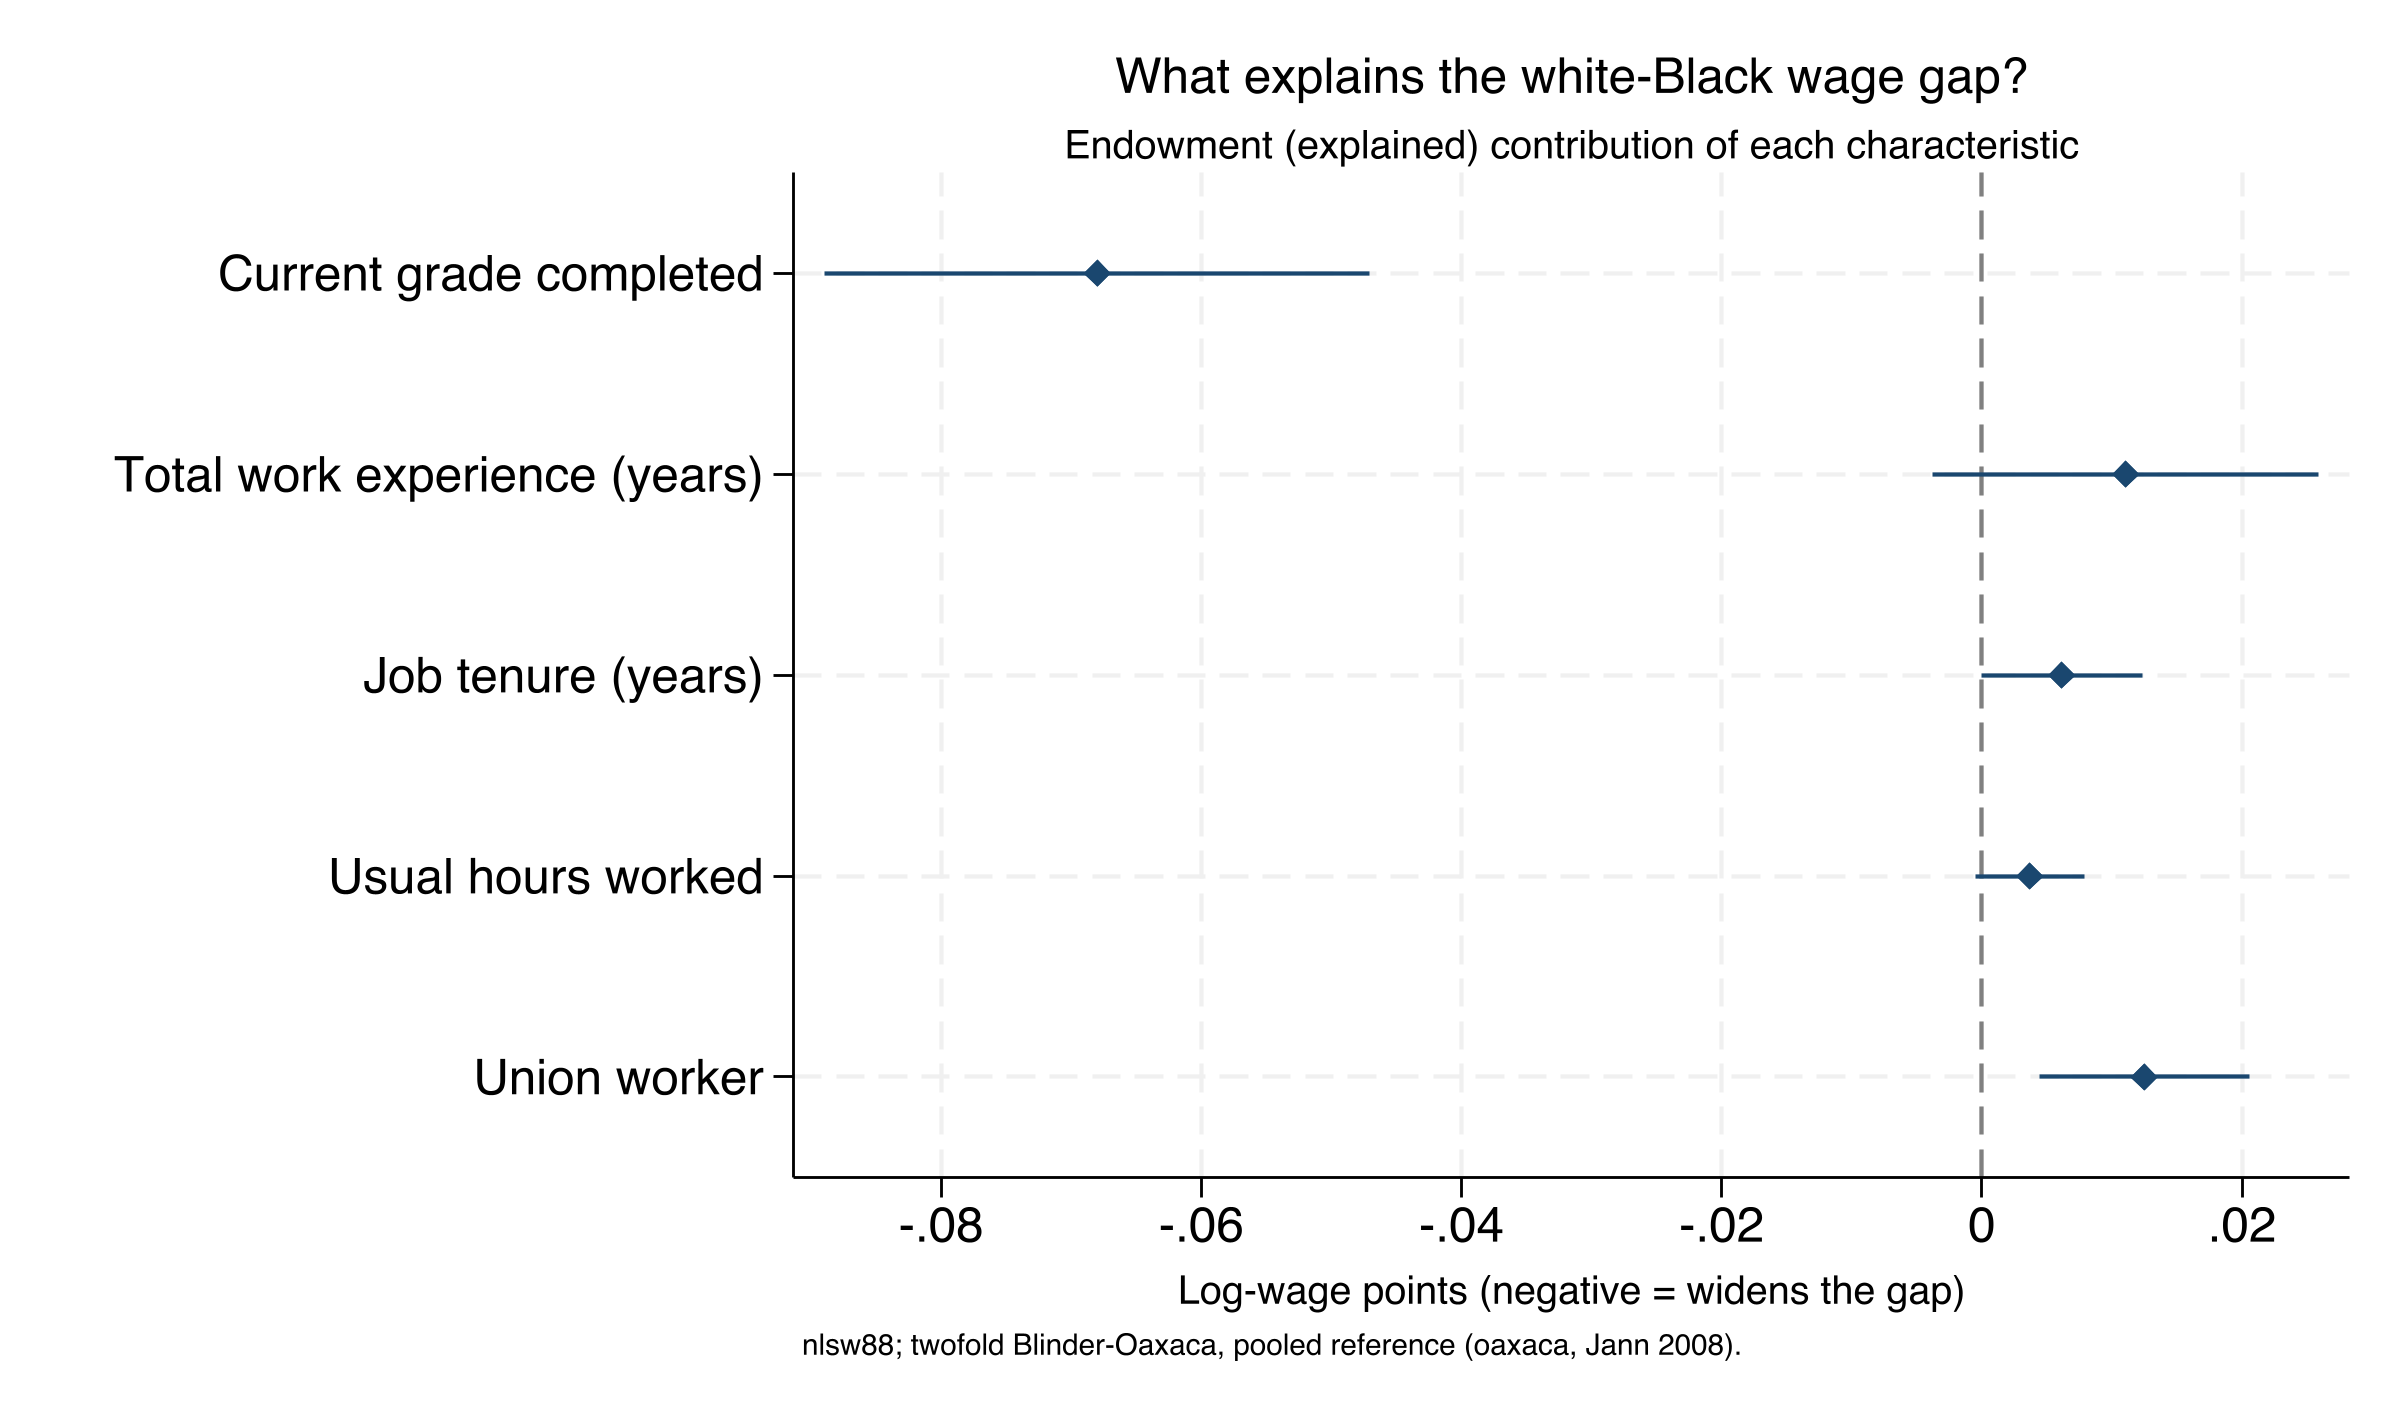
\includegraphics[width=\linewidth]{images/ch08_oaxaca.png}
\caption[The explained half of a wage gap, characteristic by characteristic]{The endowment (explained) contribution of each characteristic to the white--Black log-wage gap in \texttt{nlsw88}, from a twofold Blinder--Oaxaca decomposition with a pooled reference. A point left of zero widens the gap; right of zero narrows it. Education is the whole of the composition story; the other characteristics push the other way. The bulk of the gap, however, is \emph{unexplained} and not shown here, which is the honest limit of the method. Built by \texttt{ch08\_oaxaca.do}.}
\label{fig:ch08-oaxaca}
\end{figure*}

The commands behind this section, and the ones that turn a decomposition into a figure or a report table, all come from the Stata community; the box below collects them with their install lines.

\begin{kaobox}[frametitle={SSC toolkit: running, interpreting, and drawing a decomposition}]
Three community commands make Blinder--Oaxaca a one-sitting job, all from SSC:
\begin{itemize}
    \item \texttt{oaxaca} (Jann) \emph{runs} it: twofold or threefold, pooled or group reference, with \texttt{detail} for the per-characteristic breakdown and robust or bootstrapped standard errors. \texttt{ssc install oaxaca}.
    \item \texttt{coefplot} (Jann) \emph{draws} it: it reads \texttt{oaxaca}'s stored results directly, so \texttt{coefplot, keep(explained:)} produces Figure~\ref{fig:ch08-oaxaca} in one line. \texttt{ssc install coefplot}.
    \item \texttt{estout}/\texttt{esttab} (Jann) \emph{tables} it for a report or a \LaTeX{} appendix (Chapter~\ref{ch:sheets}). \texttt{ssc install estout}.
\end{itemize}
When the outcome is not a mean, the family extends: \texttt{oaxaca\_rif} and \texttt{rifhdreg} (Rios-Avila) decompose \emph{distributional} statistics (a median, a 90/10 ratio) via recentered influence functions, a device that turns a quantile or ratio into a per-person variable an ordinary regression can then decompose, and \texttt{mvdcmp} (Powers, Yoshioka, Yun) handles nonlinear models like logit and probit. Reach for those when the gap you care about is in the tails, not the average.
\end{kaobox}

\section{When only a causal claim will do: a working DiD kit}\label{sec:did}
Sometimes a comparison is not enough, even one decomposed characteristic by characteristic, and the question is genuinely causal: did this policy \emph{cause} this change, net of what would have happened anyway? For that question we teach one causal method end to end, difference-in-differences\index{difference-in-differences} (DiD), the right first choice because policy rollouts so often supply its ingredients: some units change, others do not, and the timing separates them. By the end of the section you will be able to build a rollout whose true effect you know, watch a one-line two-way fixed-effects regression miss it, recover it with \texttt{csdid}, and show the event-study plot before quoting the headline number, which is the sequence you need when a board member asks how you know the program caused the change rather than merely accompanied it. The core idea is intuitive, compare the before-and-after change in treated units to the before-and-after change in untreated units, so that common trends cancel out. In the simplest two-group, two-period case it is exactly one subtraction of two subtractions:
\[
\widehat{\text{DiD}}
=\underbrace{\big(\bar y^{\,T}_{\text{post}}-\bar y^{\,T}_{\text{pre}}\big)}_{\text{treated change}}
-\underbrace{\big(\bar y^{\,C}_{\text{post}}-\bar y^{\,C}_{\text{pre}}\big)}_{\text{control change}},
\]
where $\bar y^{\,T}$ and $\bar y^{\,C}$ are the mean outcomes in the treated and control groups, and the subscripts mark the periods before and after the policy. The second difference is the estimate of what would have happened anyway, so subtracting it nets it out.

Write the claim sentence a second time, now for the rollout: \enquote{the policy raised the outcome by about Z units for the units it reached.} Every phrase names a design requirement: \emph{raised} demands a counterfactual, \emph{about Z} demands a standard error, and \emph{the units it reached} limits the claim to the treated units rather than the whole population\marginnote{Statisticians call the effect on the units the policy actually reached the average treatment effect on the treated (ATT); it is what every estimator in this section targets.}. When the data cannot support a phrase, you weaken the sentence rather than stretch the design.

The modern caution fits in one paragraph and no algebra. When different units adopt a policy at different times, the once-standard two-way fixed-effects\index{two-way fixed effects} regression can mislead. That regression gives each unit a baseline level and each period a shared shock, and reads the treatment effect from what departs from both; under staggered timing it can quietly use already-treated units as if they were clean controls for later-treated ones. If the early group's effect is still evolving, that comparison is contaminated, and the estimate can even come out the wrong sign.\marginnote{\textcite{goodmanbacon2021did} is the decomposition that made this concrete: the two-way fixed-effects estimate is a weighted average of every possible 2$\times$2 DiD comparison, and the comparisons that use already-treated units as controls can subtract evolving treatment effects. In the decomposition into underlying treatment effects, some weights can be negative, which allows an overall estimate with the wrong sign.} You can avoid that contamination by reaching for an estimator that compares treated units only to units not yet treated or never treated. The \texttt{csdid}\index{csdid@\texttt{csdid}} command (Callaway and Sant'Anna) does this, building group-by-time effects you can aggregate by cohort, by calendar time, or by time since treatment. The object it estimates is the average effect for cohort~$g$ (the units that adopt in period~$g$) observed in period~$t$,
\[
ATT(g,t)=\mathbb{E}\!\left[\,Y_t(g)-Y_t(0)\;\middle|\;G=g\,\right],
\]
where $Y_t(g)$ is the outcome under treatment and $Y_t(0)$ the untreated counterfactual for the same units; only after estimating these clean pieces does the command average them into the single headline number.\sidenote{\textcite{callaway2021did} is the paper \texttt{csdid} implements; it estimates group-time average treatment effects $ATT(g,t)$ and only then aggregates. Install it and its dependency \texttt{drdid} from SSC, and note that with no never-treated units you must pass a not-yet-treated comparison group explicitly.}

Before you run any estimator, write down what the causal claim will depend on; the box below names the three assumptions, each paired with the symptom that would reveal its failure.

\begin{restson}[What the DiD claim depends on]
\begin{enumerate}
\item Parallel trends: absent the policy, treated and comparison groups would have moved together. \emph{Noticed by:} a pre-period gap in the event-study plot.
\item No anticipation: units did not change behavior ahead of their own adoption. \emph{Noticed by:} effects appearing in the periods just before treatment.
\item Clean comparisons: treated units are compared only to not-yet-treated or never-treated units. \emph{Noticed by:} construction, if the estimator is \texttt{csdid}; by nothing, if it is plain two-way fixed effects.
\end{enumerate}
\end{restson}

\subsection{A staggered rollout you can check against the truth}
The cleanest way to see the problem is to build a world where you already know the answer, then ask each estimator to recover it. We simulate a staggered adoption: 60 units followed over 12 periods, with one cohort switching the policy on at period~5, a second cohort at period~9, and a third group never treated at all.\marginnote{Simulated data with \texttt{set seed 20260704}, so the do-file \texttt{ch08\_did.do} reproduces every number here exactly. A never-treated group is the cleanest possible comparison; a well-behaved rollout usually has one, and when it does not, \texttt{csdid} falls back to the not-yet-treated units.} The treatment effect is deliberately \emph{dynamic}: it starts at 2 units in the first period of exposure and grows by one unit each period after, so for a unit five periods into treatment the effect is~7. Because we built it, we can state the truth exactly: averaged over all treated unit-periods in this panel, the true average treatment effect on the treated is~\textbf{4.83}. The early cohort climbs the ramp all the way to 9 and contributes two thirds of the treated unit-periods, while the late cohort never gets past 5; weight the two cohorts' own averages, 5.5 and 3.5, by that two-to-one exposure and you get the 4.83. Any honest estimator should land near it.

You build that world in a few lines. Each unit gets its own baseline level, and we add random disturbances and the dynamic effect to the unit-period observations. Although the variable is named \texttt{time\_fe}, its generating line draws a new value for every observation; it does not create a shock shared by all units in a period:
\par
{\footnotesize
\begin{verbatim}
set seed 20260704
set obs 60
gen unit = _n
gen cohort = cond(unit<=20, 5, cond(unit<=40, 9, 0))
gen unit_fe = rnormal(0, 2)
expand 12
bysort unit: gen period = _n
bysort period: gen time_fe = rnormal(0, 1)
gen exposure = cond(cohort==0, ., period - cohort)
gen treated  = cohort>0 & period>=cohort
gen effect   = cond(treated, 2 + (exposure), 0)
gen y = 5 + unit_fe + time_fe + effect + rnormal(0,1)
\end{verbatim}
}
You write the truth into the \texttt{effect} line: on the first treated period \texttt{exposure} is~0, so the effect is~2; four periods later \texttt{exposure} is~4 and the effect is~6. Everything else is noise the estimators must see through.

\subsection{The naive regression, and why it misleads}
The familiar first move is a two-way fixed-effects regression with a single treatment dummy, which reads as one line and reports one number:
\par
{\footnotesize
\begin{verbatim}
reghdfe y treated, absorb(unit period) vce(cluster unit)
\end{verbatim}
}
One line does three jobs: \texttt{reghdfe}\marginnote{\texttt{reghdfe} is a community command, installed by Chapter~\ref{ch:workshop}'s \texttt{01\_install.do}.} fits the regression, \texttt{absorb(unit period)} soaks up the unit and period intercepts without printing hundreds of them, and \texttt{vce(cluster unit)} asks for standard errors that let each unit's errors correlate across its own periods, the minimum honesty for repeated observations on the same units. Here is the coefficient that comes back, next to the truth:
\par
{\footnotesize
\begin{verbatim}
-----------------------------------------------------------
             y |  Coef.   Std.Err.      t     P>|t|
---------------+-------------------------------------------
       treated |  3.26     0.29     11.15     0.000
-----------------------------------------------------------
  true ATT (by construction) = 4.83
\end{verbatim}
}
The regression is confident, tightly estimated, and wrong. It reports a gain of 3.26 units when the truth is 4.83, an undercount of about a third. Nothing in the output warns you: the standard error is small and the displayed $p$-value rounds to zero, so a reader with only this table would report the contaminated number and defend it. The bias is not sampling noise; it is structural.\marginnote{The direction is diagnostic. With effects that \emph{grow} over time, the already-treated early cohort is a moving target used as a control for the late cohort, and its still-rising trend is subtracted off as if it were a common trend. That pulls the estimate below the truth. Reverse the dynamics (an effect that fades) and the same machinery can push the estimate above the truth, or past zero.}

When a program sits close to its cost-effectiveness threshold, an undercount of a third is the difference between clearing it and missing it. The naive estimate is not merely imprecise, it is biased in a direction the analyst cannot see from the regression table alone, which is exactly the failure the next estimator is built to avoid.

\subsection{The Callaway--Sant'Anna estimator, and the truth recovered}
Rather than pool, you estimate a clean effect for every cohort at every period, comparing treated units only to units not yet treated or never treated, then aggregate those pieces. The \texttt{csdid} command does this in one call, and the overall aggregation is the number to report:
\par
{\footnotesize
\begin{verbatim}
csdid y, ivar(unit) time(period) gvar(cohort) ///
    method(dripw)
estat simple
\end{verbatim}
}
To adapt this call, build \texttt{cohort} as the first treatment period for each unit and repeat that value on every row for the unit, including its pre-treatment rows. Use zero for units never treated. The cohort variable is different from \texttt{treated}, which switches on only when exposure begins; substituting that indicator for \texttt{gvar()} gives the command the wrong timing information. Check each unit's ordered records against the rollout log and confirm that the unit-period key is unique. This example assumes treatment remains in place after adoption. If a program stops and restarts, review the design before applying this setup.

The \texttt{method(dripw)} option asks for doubly-robust inverse-probability weighting\marginnote{Doubly-robust inverse-probability weighting is the safe default: it models both the outcome and the treatment odds, so the estimate stays consistent if either model is right.}. The aggregated estimate recovers the truth:
\par
{\footnotesize
\begin{verbatim}
-----------------------------------------------------------
   ATT         |  Coef.   Std.Err.    [95% Conf. Interval]
---------------+-------------------------------------------
   Simple      |  4.86     0.37       4.13       5.59
-----------------------------------------------------------
  true ATT (by construction) = 4.83
\end{verbatim}
}
Run the sense check on the pair: the estimator that keeps its comparison group clean recovers 4.86 against a truth of 4.83, inside a whisker, while the naive regression misses by more than a unit and a half in the same data. The 95\% interval covers the truth comfortably.\marginnote[-5mm]{Same panel, same noise, same seed, two estimates a unit and a half apart, and only one of them is right.} Table~\ref{tab:did-compare} lays the three numbers side by side.

\begin{table*}[htbp]
\centering
\caption[TWFE vs.\ Callaway--Sant'Anna on a known truth]{Two estimators on the same simulated staggered rollout (seed \texttt{20260704}; 60 units, 12 periods, cohorts at $t{=}5,9$, dynamic effect ramping from 2 upward). The true ATT is known by construction. Only the clean-comparison estimator recovers it; the naive regression is biased downward by contamination from already-treated units.}
\label{tab:did-compare}
{\footnotesize
\begin{tabular}{lccc}
\hline
Estimator & Estimate & Std.\ err. & vs.\ truth \\
\hline
True ATT (by construction) & 4.83 & n/a & n/a \\
Naive TWFE (\texttt{reghdfe}) & 3.26 & 0.29 & $-1.57$ \\
Callaway--Sant'Anna (\texttt{csdid}) & 4.86 & 0.37 & $+0.03$ \\
\hline
\end{tabular}
}
\end{table*}

A table of estimates cannot show a reader whether the parallel-trends assumption is credible. The box below describes the one picture that can, and we build it in the next subsection.

\begin{vizcallout}[Visualization to build: the event-study plot]
Relative time on the $x$-axis (negative is pre-treatment), the estimated effect on the $y$-axis, with 95\% confidence intervals and a vertical line at treatment. The pre-treatment points must sit flat and near zero for the parallel-trends assumption to be credible; the plot is the design's honesty check, shown before the headline number.
\end{vizcallout}

\subsection{The event study: read the pre-trend before the headline}
When you report the aggregated number alone, you hide the shape of the effect, and the credibility of the causal claim depends on that shape. Aggregating \texttt{csdid} by time since treatment, rather than into one number, gives the event study\index{event study}, which we always plot before quoting the headline:
\par
{\footnotesize
\begin{verbatim}
csdid y, ivar(unit) time(period) gvar(cohort) ///
    method(dripw)
estat event
csdid_plot, title("Event study: effect by time" ///
    " since treatment")
graph export "$figures/ch08_event.png", ///
    replace width(2400)
\end{verbatim}
}
Figure~\ref{fig:event} shows the result, and we read it in two passes. First the left half, the pre-treatment periods: those points sit flat and statistically indistinguishable from zero, with a pre-treatment average of 0.05 that is nowhere near significant, which is consistent with parallel pre-treatment trends\index{parallel trends} in this simulation. Those estimates are compatible with parallel pre-treatment trends, but their uncertainty and the program context still matter for the causal interpretation.\marginnote{Flat pre-trends are reassurance, not proof. Parallel trends is an assumption about the unobserved counterfactual, which no pre-period can verify. \textcite{rambachan2023honest} turn this into a sensitivity analysis: their \texttt{honestdid} asks how large a violation of parallel trends your headline effect could survive, and reports the answer as a breakdown value.} Then the right half, the post-treatment periods: the effect enters at about~1.8 in the first exposed period and climbs roughly one unit per period, tracing the dynamic effect we built in and passing~6 by four periods out on its way to nearly~9 at the far edge. An audience that sees the pre-trend read first will trust the ramp that follows, which is why the picture leads.

\begin{figure*}[htbp]
\centering

\includegraphics[width=\linewidth]{ch08_event.png}
\caption[Event-study plot from \texttt{csdid}]{Estimated treatment effect by time since treatment, Callaway--Sant'Anna group-time effects aggregated by exposure (simulated panel, seed \texttt{20260704}). Pre-treatment estimates (blue, to the left of period 0) sit flat and near zero, the visual test of parallel trends; post-treatment estimates (pink) climb from about 1.8 to nearly 9 at the far edge, recovering the dynamic effect built into the simulation. Read the pre-treatment estimates and their intervals first; similarity before treatment supports, but cannot establish, the counterfactual assumption needed afterward.}
\label{fig:event}
\end{figure*}

The same estimate then dresses differently for each room. The board gets one sentence in program units: \enquote{the policy raised the outcome by about five units on average, and the effect grew the longer a site had it.} The funder's paragraph keeps that sentence and adds the design in miniature: staggered rollout, comparisons only against not-yet-treated sites, flat pre-trends, and the 95\% interval. The technical appendix keeps everything the other two dropped, the event-study figure, the cohort-by-period estimates, the estimator choice, and the robustness ledger of the next subsection. Each version omits on purpose rather than diluting one paragraph three ways: the board sentence omits the interval because the board's decision does not turn on it, and the appendix omits the headline sentence because its reader is checking, not deciding.

What you should take away here is not an estimator but a sentence: the estimate is only as credible as the comparison group. The STAAR example in Appendix~\ref{app:walkthroughs} makes it concrete: a math \enquote{gain} of nearly seven points collapses to under two once the baseline is measured off a normal year instead of a pandemic trough. Beyond DiD, an evaluator meets a handful of adjacent designs, each with a Stata home: a sharp eligibility cutoff invites regression discontinuity\index{regression discontinuity} (\texttt{rdrobust}\index{rdrobust@\texttt{rdrobust}}); a single treated unit invites synthetic control\index{synthetic control} (\texttt{synth}\index{synth@\texttt{synth}}); a single site with a clear before-and-after and no control invites interrupted time series; a panel with time-varying shocks invites synthetic DiD (\texttt{sdid}). We stop at DiD on purpose, and leave the rest to the quick-reference toolbox of Appendix~\ref{app:causal} and to two excellent specialist texts, Cunningham's \emph{Causal Inference: The Mixtape} and Huntington-Klein's \emph{The Effect}.\marginnote{One section done well serves an applied evaluator better than five chapters they will not have time to read.} Figure~\ref{fig:ch08-viz-design} routes the four situations above to their Stata home so you can find the door before reading the manual behind it.

\begin{figure*}[htbp]
\centering
\begin{tikzpicture}[node distance=6mm and 10mm]
\node[io] (data) {Panel / policy\\change in hand};
\node[decision, below=8mm of data] (staggered) {Many units,\\staggered\\timing?};
\node[stage, right=16mm of staggered] (did) {DiD\\\texttt{csdid}};
\node[decision, below=9mm of staggered] (cutoff) {Sharp\\eligibility\\cutoff?};
\node[stage, right=16mm of cutoff] (rd) {RD\\\texttt{rdrobust}};
\node[decision, below=9mm of cutoff] (single) {Single\\treated\\unit?};
\node[stage, right=16mm of single] (synth) {Synthetic ctrl.\\\texttt{synth}/\texttt{sdid}};
\node[stage, below=9mm of single] (its) {One site, no\\control: ITS};

\draw[flow] (data) -- (staggered);
\draw[flow] (staggered) -- node[annot,above]{yes} (did);
\draw[flow] (staggered) -- node[annot,left]{no} (cutoff);
\draw[flow] (cutoff) -- node[annot,above]{yes} (rd);
\draw[flow] (cutoff) -- node[annot,left]{no} (single);
\draw[flow] (single) -- node[annot,above]{yes} (synth);
\draw[flow] (single) -- node[annot,left]{no} (its);
\end{tikzpicture}
\caption[Routing a design to its Stata command]{Which causal design fits which data situation, and the Stata command that estimates it. Read top to bottom and take the first \emph{yes}: staggered adoption across many units routes to difference-in-differences (\texttt{csdid}); a sharp eligibility cutoff to regression discontinuity (\texttt{rdrobust}); a single treated unit to synthetic control (\texttt{synth} or \texttt{sdid}); a single site with no control to interrupted time series. We teach only the top branch in full and route the rest to Appendix~\ref{app:causal}.}
\label{fig:ch08-viz-design}
\end{figure*}

\subsection{The robustness ledger: every path on the record}\label{ch08-sc-ledger}
Estimating the headline is the fast part; defending it is where the unreported specifications pile up. Between the first \texttt{csdid} call and the final table, an analyst typically runs a dozen variants: an alternative comparison group, a dropped cohort, a different aggregation, a placebo outcome. The garden of forking paths grows exactly there, because memory keeps the flattering runs and loses the rest. So we keep a robustness ledger, this chapter's instance of the tracking-spine pattern of Chapter~\ref{ch:workshop}: one row per specification run, recording the date, the specification, the sample size, the estimate, the standard error, why the run was made, and whether it was kept or dropped and on what grounds.\marginnote{A robustness-ledger row from this chapter's example: \texttt{2026-07-04, csdid dripw baseline, N=720, 4.86 (0.37), primary spec per memo, kept}.}

The ledger converts the forking paths from a temptation into a record. Every path taken is on the page, so the final report can state plainly which specifications were run and how the headline held up across them, and a hostile reviewer's \enquote{what else did you try} has a documented answer instead of a reconstructed one. It also writes the robustness appendix almost by itself: kept rows become the appendix table, dropped rows become its footnotes. Section~\ref{sec:prereg} supplies the companion discipline, since the pre-analysis memo states the paths in advance and the ledger records the ones actually walked.

\subsection{Choosing comparison units transparently when N is small}\label{ch08-sec:twins}
The synthetic-control machinery presumes a donor pool large enough to average, but an embedded evaluator is often handed the opposite: one treated site and a dozen candidate comparisons, where a formal synthetic weight would overfit and no reader could audit the choice. Instead of reaching for a black-box optimizer, we suggest you start transparently: rank the candidate units by how closely they resemble the treated site on the covariates that matter, and state the ranking out loud. \textcite{abadie2021synth} makes the same point from the other direction: a synthetic control is credible only when its donor pool contains genuinely comparable units, chosen before the outcome is seen, not reverse-engineered to fit the treated unit's trajectory. Picking the comparison group transparently is the small-N analogue of that discipline. In the rest of this subsection we install the tool that does the ranking and work one example end to end, so you finish with a shortlist you can put in front of a client and defend a year later, rather than a set of weights no one in the room can check.

The \texttt{twinmatch}\index{twinmatch@\texttt{twinmatch}} command ranks \emph{policy twins}: the candidate units nearest the treated one in Mahalanobis\index{Mahalanobis distance} distance on a stated covariate set. The distance from candidate unit~$i$ to the treated unit~$t$ is
\[
d(i,t)=\sqrt{\,(\mathbf{x}_i-\mathbf{x}_t)^{\!\top}\,S^{-1}\,(\mathbf{x}_i-\mathbf{x}_t)\,},
\]
where $\mathbf{x}_i$ and $\mathbf{x}_t$ are the two units' covariate vectors and $S^{-1}$ is the inverse covariance matrix, which rescales each covariate by its spread and de-correlates them so no single wide-ranging variable dominates the ranking. It is a donor-selection helper, not an estimator, so it hands the evaluator a defensible shortlist to reason about rather than a number to report. Install it alongside the other book tools:
\par
{\footnotesize
\begin{verbatim}
local gh "https://raw.githubusercontent.com/ericabooth"
net install twinmatch, ///
    from("`gh'/twinmatch-stata-public/main/") replace force
\end{verbatim}
}
The mechanics are quickest to see on the built-in \texttt{auto} data, treating one car as the \enquote{treated} unit and asking which others most resemble it on mileage, price, and weight:
\par
{\footnotesize
\begin{verbatim}
sysuse auto, clear
twinmatch mpg price weight, id(make) ///
    treated("Volvo 260") ntwins(3) gen(d260)
* the colon runs an extended macro function: take word 1
local nearest : word 1 of `r(twins)'
display "nearest twin: `nearest'"
\end{verbatim}
}
The ranked twins come back as \texttt{Peugeot 604} (distance 0.57), \texttt{Linc.\ Versailles} (0.90), and \texttt{Audi 5000} (1.01), and \texttt{r(dists)} stores the distances so a reader can see how much closer the first twin is than the third. Read as a policy exercise, this is the move an evaluator makes before any formal synthetic control: name the covariates that define comparability, let the distance rank the candidates, and put the shortlist in front of the client so the comparison group is chosen in the open. The twins then become the donor pool a formal method draws on, or, when N is too small even for that, the handful of case-study comparisons the evaluator reasons about directly.\marginnote{\texttt{twinmatch} v0.1.0 selects and ranks only; it does not weight the twins, test balance, or estimate an effect, so the twin list is a starting point, not a result. Collinear covariates are dropped from the distance after a printed warning, which is a feature: a metric built on redundant columns would exaggerate closeness.} Give the shortlist its own ledger row: record the covariate set, the ranked twins, and the date the list went to the client, so a later reader can verify the donor pool was fixed before the outcome data arrived.

When the design does grow into a formal synthetic control, the reporting question becomes uncertainty, and the field has moved past answering it with placebo permutations alone, which re-estimate the effect as though each untreated unit had been treated and ask where the real one ranks. \textcite{cattaneo2021prediction} derive prediction intervals for synthetic-control estimates that guarantee finite-sample coverage, and \textcite{cattaneo2025scpi} ship them in the cross-platform \texttt{scpi} package for Stata, R, and Python. Select the donor pool transparently with \texttt{twinmatch}, estimate the synthetic control, and \texttt{scpi} then hands you an interval a board can read the way it reads the ROI range of Section~\ref{sec:roi}: a point estimate with error bars rather than a single line asserted with false confidence.

\subsection{The frontier: from ``did it work'' to ``for whom, and how sure''}\label{ch08-sec:frontier}
Two questions remain just beyond what this book ships, and both are where an applied evaluator's field is moving. The first is heterogeneity: an average effect answers \enquote{did it work} but hides \enquote{for whom,} and a program director planning who to enroll next needs the second answer more than the first. The second is honesty about the parallel-trends assumption that every DiD requires. We treat both as frontier, meaning we describe the method and cite it plainly, then say what the evaluator gains and what it costs, without pretending the book hands you a turnkey command for either.

The \enquote{for whom} question has a modern answer in the causal-forest literature. \textcite{athey2016recursive} adapt regression trees to split a sample not by outcome but by \emph{treatment effect}, so the algorithm itself finds the subgroups where a program helps most and least; \textcite{wager2018forests} extend this to random forests with valid confidence intervals for the estimated effect at each covariate profile. The payoff for an evaluator is exactly the payoff of the pre-registered subgroup analysis in Section~\ref{sec:prereg}, but discovered rather than declared: instead of guessing which two subgroups to test, the forest surfaces the heterogeneity the data actually contain.\marginnote{The National Study of Learning Mindsets \parencite{yeager2019mindset}, described in Chapter~\ref{ch:embedded}, is the canonical case: its average effect was small, and the \enquote{for whom} was the whole finding.} The cost is discipline: a forest that searches thousands of splits will find spurious heterogeneity unless the analysis is split into a discovery sample and a confirmation sample, which is the garden-of-forking-paths problem of Section~\ref{sec:prereg} restated in machine-learning form; the discovery-confirmation split is itself a line worth writing into the pre-analysis memo before the forest runs. \textcite{athey2017state} survey where this and the rest of applied causal machine learning stand, and their paper maps the territory we stop short of here.

When a skeptic presses on a headline effect, you need more than the margin note beside the event study had room for. Flat pre-trends are reassuring but they cannot prove parallel trends, because the assumption is about an unobserved counterfactual no pre-period can see. \textcite{rambachan2023honest} convert this from a yes-or-no test into a sensitivity analysis: given the pre-trend you observe, how large a violation of parallel trends would it take to overturn your headline effect, and is that violation plausible? Their \texttt{honestdid}\index{honestdid@\texttt{honestdid}} reports the answer as a breakdown value, the size of departure at which the confidence interval first admits a null effect. The gain for an evaluator is a defensible sentence to a skeptical board: \enquote{the effect survives any pre-trend violation up to twice the largest one we observe,} which is a stronger claim than \enquote{the pre-trends look flat.} The cost is that you must state in advance what class of violations to consider. \textcite{roth2023trending} place this sensitivity work in the modern DiD literature, the same body of work that gave us the Callaway--Sant'Anna estimator we ran above.

Beyond those two, a related frontier tightens the comparison group itself. Kernel balancing, from \textcite{hazlett2020kernel}, chooses weights on the comparison units so that treated and comparison groups match not just on the means of the covariates but on many transformed versions of them at once, which guards against the omitted nonlinearity that ordinary matching misses. For an evaluator working with observational comparison groups, \texttt{kbal}\index{kbal@\texttt{kbal}} is the natural next tool after the transparent twin-selection of Section~\ref{ch08-sec:twins}: twins pick the donor pool in the open, kernel balancing weights it to remove residual imbalance a distance ranking alone would leave behind.

\begin{kaobox}[frametitle=Existing tool: kernel balancing with \texttt{kbal}]
\textbf{Use what exists:} kernel balancing is implemented by its author. Hazlett's \texttt{kbal} is on CRAN for R, with a Stata version distributed through his site and GitHub rather than SSC, so the install is a download rather than one \texttt{ssc install}. Either version takes a treated indicator and covariates, chooses comparison-unit weights that balance a kernel expansion of the covariates rather than their raw means, and returns the weights with a balance table. When you use it, report the effective sample size the weights imply, so a reader sees how much of the comparison group the balancing actually kept.
\end{kaobox}

\begin{kaobox}[frametitle=When the next question is \enquote{did it work \emph{through} attendance?}]
A headline effect invites a mechanism question, and the reflex answer, rerunning the regression with attendance added as a control, is quietly wrong. Attendance is measured \emph{after} treatment begins, so controlling for it compares treated and untreated people who reached the same attendance for different reasons, and that comparison is no longer protected by the design. The reporting choice depends on the question the evidence can support. You can begin by treating the mediator as an outcome in its own right: \enquote{the program raised attendance by X} is a clean claim with its own claim sentence. If the client needs the formal decomposition, direct versus indirect effects, say plainly that it requires assumptions beyond anything in this chapter and budget for the specialist treatment: \textcite{vanderweele2015explanation} is the standard reference, and \textcite{huber2023causal} covers the estimation side.
\end{kaobox}

\section{What did it cost, what did it return}\label{sec:roi}
Answer the money question with a range a board can plan against, not a single ratio that quietly hinges on one shaky input. Funders ask the cost question as directly as the effect question, and it deserves the same care. By the end of the section you will be able to price a program as a distribution rather than a ratio, reporting a median return, a plausible range around it, the share of draws that clear break-even, and a ranked list of which assumptions are doing the work, which is the version a board can act on when it decides whether to fund a second cohort. Start a cost-effectiveness or return-on-investment\index{return on investment} analysis by fixing the accounting perspective: whose costs and whose benefits count, the funder's, the participant's, or society's, because the answer changes with the frame. You discount future benefits to present value,\marginnote{The discount rate is a value judgment expressed as a number. U.S. federal guidance (OMB Circular A-94) long anchored on 7\%, while much of the climate literature argues for rates near 2--3\% precisely because a high rate all but erases benefits that arrive decades from now. Report your result at two or three rates rather than defending one.} and because every input is uncertain, you run a Monte Carlo\index{Monte Carlo simulation} simulation, which propagates that uncertainty into a distribution of returns rather than a single misleadingly precise number.

\subsection{A worked ROI: from point estimate to a distribution}
Take the training program from the DiD example and price it. Suppose the effect we just estimated translates to an annual earnings gain per participant, that the program costs a fixed amount per seat, and that the gain persists for several years but is discounted back to today. Here ROI is net discounted benefits divided by costs; the benefit-cost ratio instead divides gross benefits by costs. For an honest ROI, you draw each uncertain input from a distribution ten thousand times and report the spread:
\par
{\footnotesize
\begin{verbatim}
set seed 20260704
local reps 10000
gen roi = .
forvalues i = 1/`reps' {
    local gain  = rnormal(3000, 900)   // annual $ gain
    local cost  = rnormal(4200, 400)   // $ per seat
    local years = 3 + int(3*runiform())// 3-5 yr persistence
    local disc  = 0.02 + 0.05*runiform()
    local pv = 0
    forvalues t = 1/`years' {
        local pv = `pv' + `gain'/(1+`disc')^`t'
    }
    quietly replace roi = (`pv'-`cost')/`cost' in `i'
}
summarize roi, detail
\end{verbatim}
}
The Monte Carlo returns not one ROI but ten thousand, and the summary is what you report:
\par
{\footnotesize
\begin{verbatim}
-----------------------------------------------------------
        roi |  Percentiles      Smallest
        10% |    0.40          -1.61
        25% |    0.88
        50% |    1.47          Mean       1.57
        75% |    2.19          Std.Dev.   0.97
        90% |    2.86
-----------------------------------------------------------
\end{verbatim}
}
Translate before you believe: a median ROI of 1.47 means the program returns about \$1.47 in net discounted earnings per dollar spent, and at the tenth percentile, 0.40, even a pessimistic draw of the inputs still returns forty cents on the dollar in net terms. Reporting \enquote{ROI of about 1.5, with a plausible range from roughly 0.4 to 2.9} tells a board how much of the bet is safe, which the bare 1.47 never could.\marginnote{The number a board actually wants is often the break-even probability: the share of the ten thousand draws with ROI above zero. Here the reported tenth-through-ninetieth percentiles all clear zero, so discounted benefits exceed costs across most simulated draws, though the full distribution still contains a thin loss tail below the tenth percentile, which is worth reporting rather than rounding away.}

You draft the money claim exactly as you drafted the causal one, and dress it for the same three rooms. Written before the simulation runs, the claim sentence reads: \enquote{each dollar spent returns about \$1.50 in net discounted earnings, and the return stays positive across nearly all plausible assumptions.} The board hears the break-even probability in words. The funder's paragraph adds the median, the tenth-to-ninetieth range, and one line naming the two inputs the tornado chart of the next subsection says are worth arguing about. The technical appendix records the input distributions, the seed, the draw count, and the independence caveat, because a technical reader's first question is what was assumed, not what was found. Give each rerun with a changed assumption set its own row in the robustness ledger of Section~\ref{ch08-sc-ledger}\marginnote{A favorable ROI reached by quiet tuning of the persistence horizon is the money version of a fished subgroup.}.

\begin{vizcallout}[Visualization to build: the tornado chart]
A tornado diagram showing how the ROI estimate moves as each key assumption varies across its plausible range, bars sorted longest at the top. It tells stakeholders which assumptions actually drive the result, so the debate can focus on the two or three inputs that matter instead of all of them.
\end{vizcallout}

\subsection{The tornado: which assumption is driving the answer}
A board reads the distribution for how confident to be, and the tornado for \emph{what to argue about}. We hold every input at its central value, then swing one input at a time to the low and high ends of its plausible range and record how far the ROI moves. Sorting those swings longest-first produces Figure~\ref{fig:tornado}. Read the order first: the annual earnings gain and the persistence horizon move the ROI by far more than the discount rate or the per-seat cost do. A board that reads this stops litigating the discount rate, which barely matters here, and concentrates its scrutiny on the earnings-gain estimate, which is both the longest bar and the one our DiD design was built to pin down.

\par
{\footnotesize
\begin{verbatim}
graph hbar (asis) swing, over(input, sort(1)) ///
    title("Tornado: what moves the ROI")
graph export "$figures/ch08_tornado.png", ///
    replace width(2400)
\end{verbatim}
}

\begin{figure*}[htbp]
\centering

\includegraphics[width=\linewidth]{ch08_tornado.png}
\caption[ROI tornado from a Monte Carlo]{Sensitivity of the return-on-investment estimate to each uncertain input, one bar per input, longest at the top (simulated, seed \texttt{20260704}). Each bar is the swing in ROI as that input alone moves from the low to the high end of its plausible range with all others held at center. The earnings gain and the persistence horizon dominate; the discount rate barely registers. Read it and you can tell a board which two numbers are worth arguing about.}
\label{fig:tornado}
\end{figure*}

When ROI pricing becomes routine, the box below supplies the shortcut: the whole simulation, tornado sweep included, as one installable command.

\begin{kaobox}[frametitle=Package Integration: \texttt{roisim}]
We wrote the loop out by hand so you can see the machinery once, but when you price programs every month you want the same answer in one line. \texttt{roisim}\index{roisim@\texttt{roisim}} takes the effect estimate and its standard error, a cost range, and the discount and horizon ranges, draws each input ten thousand times, and returns the ROI percentiles, the break-even probability, and the tornado sweep as saved results. Install it from the book's repository:
\par
{\footnotesize
\begin{verbatim}
local gh "https://raw.githubusercontent.com/ericabooth"
net install roisim, ///
    from("`gh'/roisim-stata-public/main/") replace force
\end{verbatim}
}
Use the same effect, discount, and horizon settings, but note the change in cost distribution: the command below draws costs uniformly over the stated range, whereas the hand-coded loop uses a Normal distribution:
\par
{\footnotesize
\begin{verbatim}
roisim, effect(3000) se(900)      ///
    costlow(3800) costhigh(4600)  ///
    discountrange(0.02 0.07)      ///
    horizonrange(3 5)             ///
    reps(10000) seed(20260706)
display "median ROI = " r(p50)
display "Pr(ROI>0)  = " r(prpos)
\end{verbatim}
}
The command reports a median ROI of about 1.48 and a break-even probability \texttt{r(prpos)} of 0.97, which lands on the hand-coded median of 1.47 and confirms in one number what the percentile table said the long way: discounted benefits exceed costs across nearly all draws under these assumptions. \texttt{roisim} also prints the tornado sweep, and it ranks the inputs exactly as Section~\ref{sec:roi} argued, effect first, then horizon, with cost and discount far behind, so the saved \texttt{r(tornado)} matrix feeds Figure~\ref{fig:tornado} directly.\marginnote{The v0.1.0 caveat to keep visible: effect draws are Normal and cost draws Uniform, drawn independently, so \texttt{roisim} does not yet model correlated inputs. When two assumptions move together (a larger effect that also costs more to deliver), the independent draws overstate how much the tails cancel, and the hand-coded loop, where you control the joint draw, remains the honest fallback.}
\end{kaobox}

An ROI with visible uncertainty is more actionable than a point estimate, not less. Present the distribution and you have answered the money question without overpromising, handing the funder a number it can plan against rather than one that will embarrass everyone in two years.

\section{Subgroups without fishing}\label{sec:prereg}
The fastest way to manufacture a false finding is to search subgroups until one turns up significant. The guard is simple: decide what to test before you see the data, so a reader can tell a planned subgroup from one you went looking for after the fact. We pre-register\index{pre-registration} the primary outcomes, the covariates, and the planned subgroup analyses in a timestamped, version-controlled document in the project repository,\marginnote{A git commit is a timestamp only you can vouch for. For a stamp a skeptic will accept, register the plan externally: OSF (\texttt{osf.io}) takes a full analysis plan and freezes it, while AsPredicted asks nine short questions and suits a lean evaluation shop that would otherwise register nothing.} and we label anything discovered afterward as exploratory rather than confirmatory. This is the same commitment device Chapter~\ref{ch:embedded} recommended against political pressure, now pointed at our own analytic temptations.

In an embedded shop the plan is usually a memo, not a filing, and a page suffices: the claim sentence from Section~\ref{sec:comparisons} with its blanks still visible, the primary outcome and the units it is measured in, the comparison group and why, the two or three subgroups with the reason each is worth testing, and the date. Send it to the program director before the outcome data arrive and keep the sent copy.\marginnote{A dated memo sitting in two inboxes is a commitment a skeptical reader can check, and it costs an afternoon where a registry filing can stall for weeks. The registry remains the stronger stamp when the stakes warrant it; the memo is the version a lean shop will actually write.} The robustness ledger of Section~\ref{ch08-sc-ledger} is the memo's mirror image: the memo binds the paths in advance, the ledger records the ones walked, and together they let an evaluator say, with documents rather than assurances, that the finding was not fished.

Why bind your own hands? An embedded shop trades on credibility, and credibility does not survive a reputation for finding whatever the client hoped for. Pre-register, and a reader can trust even the simple comparisons of Section~\ref{sec:comparisons}, because the primary outcome was on record before the data could tempt anyone. Every claim in this chapter leans on that quiet discipline.

\subsection{Estimating subgroup effects without being fooled by noise}\label{ch08-sc-shrinkfx}
Pre-registration guards \emph{which} subgroups you test; it does not guard how you read the six numbers that come back. Split any sample six ways and the smallest cells produce the noisiest estimates, so the most dramatic subgroup effect on the page is usually the one standing on the least data, and it is exactly the number a program director wants to fund.\marginnote{Statisticians call this the winner's curse: select the largest estimate from a set and you have selected, in expectation, the luckiest one, not the truest.} Chapter~\ref{ch:trust} met this same shape of problem in site rates and answered it with shrinkage; the identical arithmetic works on treatment effects.

To show it, we simulate a program whose true effects genuinely differ across six subgroups, from 2.9 points in the largest to 7.4 in the smallest, with subgroup sizes running from 1{,}209 people down to 122. One regression per subgroup gives the raw estimates; a precision-weighted average gives the pooled effect; and the spread of the estimates beyond what their standard errors explain gives the between-group variance, $\hat\tau^2$. Each subgroup then keeps its own estimate in proportion to its reliability, exactly as \texttt{rateshrink} does for rates:
\par
{\footnotesize
\begin{verbatim}
forvalues g = 1/6 {
    quietly regress y treat if grp==`g'
    post `h' (`g') (r(N)) (_b[treat]) (_se[treat])
}
* ...pooled effect B and between-group variance tau2, then:
gen double rel   = `tau2'/(`tau2' + se^2)
gen double b_shr = rel*b + (1-rel)*`B'
\end{verbatim}
}
The run reports a pooled effect of 4.28 and $\hat\tau^2 = 0.44$, and the table is the whole lesson:
\par
{\footnotesize
\begin{verbatim}
  | grp      n      b     se    rel   b_shr |
  |-----------------------------------------|
  |   1   1209   3.47   0.56   0.58    3.81 |
  |   2    734   4.55   0.73   0.45    4.40 |
  |   3    440   4.37   0.93   0.34    4.31 |
  |   4    312   4.47   1.17   0.24    4.32 |
  |   5    183   7.63   1.57   0.15    4.78 |
  |   6    122   5.74   1.78   0.12    4.46 |
\end{verbatim}
}
Read row 5 first, because it is the row a meeting would seize on: a 7.63-point effect, nearly double everyone else's. Its subgroup has 183 people, its reliability is 0.15, and shrinkage cuts it to 4.78. The largest subgroup keeps most of its own estimate (3.47 moves only to 3.81, reliability 0.58), and the reliability column falls with size exactly as it did in Chapter~\ref{ch:trust}'s site table: sample size buys the right to your own number. Shrinkage is not free, and say so when you present it: in this simulation subgroup 5's true effect is 6.5, so the shrunken 4.78 undershoots a genuinely large effect. The defense is the same one Chapter~\ref{ch:trust} used: report the raw column, the shrunken column, and the reliability beside them, so the reader sees how much evidence stands behind each row rather than a single confident-looking number. The companion \texttt{ch08\_subgroups.do} reruns all of it, and asserts that every shrunken estimate lies between its raw value and the pool.

When you want the data to \emph{find} the subgroups rather than test the ones you declared, the causal-forest work already cited in Section~\ref{ch08-sec:frontier} is the method, and the tooling has reached Stata: Stata~19's \texttt{cate} estimates group-average effects for prespecified groups and for data-driven groupings of the predicted effect, and the community \texttt{ddml} route appears in Appendix~\ref{app:causal}. \textcite{huber2023causal} treats these estimators at book length, estimator by estimator, for graduate econometrics courses in R; we stop earlier on purpose, because an embedded evaluator usually knows which subgroups the program logic names before any algorithm looks, and the step the estimator-first treatments skip is the one this section adds: what to do honestly with the small handful of noisy subgroup numbers you already have.

\paragraph{Where this leaves you.} You leave this chapter able to match a claim to its design: describe comparisons with the sense-check reflex, run a defensible difference-in-differences that recovers the truth when the naive regression cannot, price a program with honest uncertainty, shrink subgroup estimates to the credibility their sizes support, and pre-register your way past the garden of forking paths. When the design question gets harder, the same discipline extends: choose a small-N comparison group in the open with policy twins before reaching for a formal synthetic control, and name the field's frontier honestly, heterogeneous-effect forests for the \enquote{for whom} question and parallel-trends sensitivity analysis for the \enquote{how sure,} even where the book stops short of shipping a command for each. Two working documents accompany all of it: the dated pre-analysis memo that fixes the claim before the data can tempt you, and the robustness ledger that keeps every specification on the record. The causal toolbox continues in Appendix~\ref{app:causal}, and two specialist texts, Cunningham's \emph{The Mixtape} and Huntington-Klein's \emph{The Effect}, are where to go when a design outgrows this chapter. Part~IV turns to the other half of the job, communicating it so the people who need it can actually use it, beginning with graphics in Chapter~\ref{ch:graphs}.

\section*{Exercises}\addcontentsline{toc}{section}{Exercises}
\begin{enumerate}
  \item \emph{Try it on your own data.} Take a policy your own panel rolls out at different times, build a cohort variable that records each unit's adoption period, and run \texttt{csdid} with \texttt{estat simple}. Then apply the sense check: does the aggregated effect match the direction and rough size a program director would expect, and if not, hunt the merge or units error before you trust the number.
  \item Rerun the companion do-file \texttt{ch08\_did.do} unchanged and confirm the naive \texttt{reghdfe} coefficient returns 3.26 and the \texttt{csdid} aggregate returns 4.86 against the true ATT of 4.83. Then change \texttt{set seed 20260704} to a new seed, rerun, and report how far each estimator moves from the truth.
  \item \emph{Predict, then check.} Before you run anything, write down whether the naive two-way fixed-effects estimate will land above or below the true ATT when the built-in effect \emph{grows} over time; then run the regression and confirm the sign of the gap you predicted.
  \item \emph{Break it and see.} In \texttt{ch08\_did.do}, recode the never-treated group so its cohort variable takes a value instead of zero, rerun \texttt{csdid}, and watch the aggregate drift off 4.83 once the clean comparison group is gone; restore the zero and confirm the truth returns.
  \item Rerun the ROI Monte Carlo with the earnings gain drawn from \texttt{rnormal(3000, 900)}, then predict whether widening that gain's standard deviation to 1500 will move the median ROI or mainly fatten the loss tail below the tenth percentile; rerun and check your prediction against \texttt{summarize roi, detail}.
  \item \emph{One line against the long way.} Install \texttt{roisim} and rerun the worked ROI with \texttt{effect(3000) se(900) costlow(3800) costhigh(4600) discountrange(0.02 0.07) horizonrange(3 5) seed(20260706)}; confirm \texttt{r(p50)} comes out near the hand-coded median of 1.47 and read the printed tornado sweep, then say in one sentence which input a board should argue about first and why the discount rate is not it.
  \item \emph{Start the ledger.} For exercise 1, keep a robustness ledger with one row per \texttt{csdid} variant you run (date, specification, N, estimate, standard error, why run, kept or dropped). Run at least three variants, an alternative comparison group, a dropped cohort, and a placebo outcome, then write the one-sentence board version of what the ledger shows and the one-line appendix footnote for the variant you dropped.
\end{enumerate}
